\documentclass[11pt]{article}
\usepackage{arXiv}
\usepackage{amsmath,amssymb,amsthm,booktabs,array}
\usepackage{tikz}\usetikzlibrary{decorations.pathreplacing}
\hypersetup{colorlinks=true,linkcolor=blue!60!black,citecolor=blue!60!black,urlcolor=blue!60!black}
\newcommand{\R}{\mathbb{R}}\newcommand{\N}{\mathbb{N}}
\newcommand{\PA}{P_{\!A}}\newcommand{\EA}{E_{A}}\newcommand{\KA}{K_{\!A}}
\newcommand{\pr}[1]{\pi_{#1}}
\DeclareMathOperator{\supp}{supp}
\title{Applying an arbitrary matrix across the modes of a downward closed set:\\ the product-set sweeps}
\author{Exploration notes (worktree \texttt{fft\_paper\_apply}), 30 September 2026}
\date{}
\begin{document}
\maketitle
\begin{abstract}
Let $A\subset\{0,\dots,n-1\}^m$ be downward closed and $M\in\R^{n\times n}$ arbitrary. The FNT / lpFun
route computes $y=\PA(M\otimes\cdots\otimes M)\EA c$ by tube sweeps of the unpivoted LU factors of $M$ on the
tubes of $A$; it is exact only when that LU exists, and pivoting is impossible because the row index is the
polynomial degree. This note explains, from the ground up, the simplest exact alternative that works for every
$M$: sweep $M$ itself, direction by direction, but keep the $k$-th intermediate result on the
\emph{product set} $\pr{\le k}(A)\times\pr{>k}(A)$ instead of on $A$. Each tube then receives the rectangular
leading block $M[0{:}L_{\rm out},\,0{:}L_{\rm in}]$. We prove exactness (the needed-set principle), give the
algorithm, the cost ($\sum_k|\pr{\le k}A|\,|\pr{\ge k}A|$ multiply--adds, $1.1$--$1.7\times$ the FNT for $\ell^2$ balls
with $m\le4$), the rounding-error bound (no growth factor, no pivots), and the relation to LU, bounded-delay
pivoting, $QR$ and the solve.
\end{abstract}

\section{Setting and the question}
Fix $m\ge1$ and $n\ge1$ and write $B=\{0,\dots,n-1\}^m$ for the box of multi-indices. A set $A\subset B$ is
\emph{downward closed} if $\beta\le\alpha$ componentwise and $\alpha\in A$ imply $\beta\in A$. Vectors indexed by
$B$ are $m$-dimensional arrays; $\EA:\R^{A}\to\R^{B}$ extends a vector on $A$ by zeros and $\PA=\EA^{\!\top}$
restricts to $A$. For a matrix $M\in\R^{n\times n}$ the \emph{mode-$d$ product} $M_{(d)}$ applies $M$ along
coordinate $d$ of a box array,
\[
 (M_{(d)}v)(\beta)=\sum_{\gamma=0}^{n-1} M_{\beta_d,\gamma}\; v(\beta_1,\dots,\beta_{d-1},\gamma,\beta_{d+1},\dots,\beta_m),
\]
and $M^{\otimes m}=M_{(m)}\cdots M_{(1)}$ (the mode products in different directions commute). The operator we
want is the cropped Kronecker product
\begin{equation}\label{eq:KA}
 \KA(M):=\PA\,M^{\otimes m}\,\EA\ \in\R^{|A|\times|A|},\qquad y=\KA(M)\,c .
\end{equation}
It is the principal submatrix of $M^{\otimes m}$ indexed by $A$: ``apply the 1D operator $M$ in every direction
to a polynomial whose coefficients live on $A$, and keep the coefficients in $A$''. Everything below holds
verbatim for different matrices $M^{(d)}$ in different directions (and different $n_d$); we write one $M$ for
readability.

\paragraph{Tube sweeps.} A \emph{tube} of $A$ in direction $d$ is the set of points of $A$ that differ only in
coordinate $d$. Because $A$ is downward closed every tube is a prefix $\{0,\dots,L-1\}$ of its coordinate. A
\emph{sweep} of a matrix $F$ in direction $d$ applies $F[0{:}L,0{:}L]$ to every tube. The FNT/HP21 principle
is: for $M=LU$ (no pivoting) the two sweeps ``$U$ in every direction, then $L$ in every direction'' compute
$\KA(M)c$ exactly at cost $2m$ sweeps. This is what lpFun's \texttt{Transform.apply} does.

\paragraph{The question.} What do we do when $M$ has no unpivoted LU, or an unstable one? We cannot permute
rows ($M=PLU$): the row index is the degree, and $A$ is defined in terms of it. The present note answers with
the cheapest exact route that needs no factorisation at all.

\section{The naive two-step and why it fails}\label{sec:naive}
The tempting algorithm is: sweep $M[0{:}L,0{:}L]$ itself in direction $1$ on the tubes of $A$, then in direction
$2$, and so on. This is \emph{not} $\KA(M)c$ unless $M$ is triangular. The smallest counterexample has $m=2$,
$n=2$, $A=\{(0,0),(1,0),(0,1)\}$ (the box minus its corner $(1,1)$), $M=\begin{psmallmatrix}a&b\\ c&d\end{psmallmatrix}$.
The exact operator gives, at the point $(1,0)$,
\[
 y(1,0)=\sum_{\beta\in A} M_{1,\beta_1}M_{0,\beta_2}\,c_\beta
       = c\,a\;c_{00}+d\,a\;c_{10}+c\,b\;c_{01}.
\]
The naive route first sweeps direction $1$: the column $\beta_2=0$ is a tube of length $2$ and gets the full
$M$, the column $\beta_2=1$ is a tube of length $1$ and gets $M[0{:}1,0{:}1]=a$:
\[
 v(0,0)=a\,c_{00}+b\,c_{10},\quad v(1,0)=c\,c_{00}+d\,c_{10},\quad v(0,1)=a\,c_{01},\qquad v(1,1)\ \text{not computed}.
\]
Then it sweeps direction $2$: the row $\beta_1=1$ is a tube of length $1$, so $y(1,0)=a\,v(1,0)=a\,c\,c_{00}+a\,d\,c_{10}$.
The term $c\,b\,c_{01}$ is missing. It would have come from $v(1,1)=c\,c_{01}$, the value the first sweep pushed
\emph{out of $A$} (row $1$ of $M$ acting on the column $\beta_2=1$), which the second sweep then needs (column $1$
of $M$ acting on the row $\beta_1=1$). The missing coefficient $M_{1,0}M_{0,1}$ is exactly a
``lower entry followed by an upper entry''; if either vanishes the term disappears, which is why triangular
matrices never have this problem.

\section{The idea in pictures}\label{sec:pict}
This section says the same thing as Sections~\ref{sec:needed}--\ref{sec:algo} without notation. Think of $c$ as an
array on the whole box that is zero outside the staircase $A$. ``Apply $M$ in every direction'' means: take every line
of the array parallel to axis~1, multiply it by $M$ as a vector; then every line parallel to axis~2; and so on; at the
end keep the entries inside $A$. Doing this on the full box is obviously correct, only expensive. The question is
which entries of the intermediate arrays can be thrown away.

\begin{figure}[ht]\centering
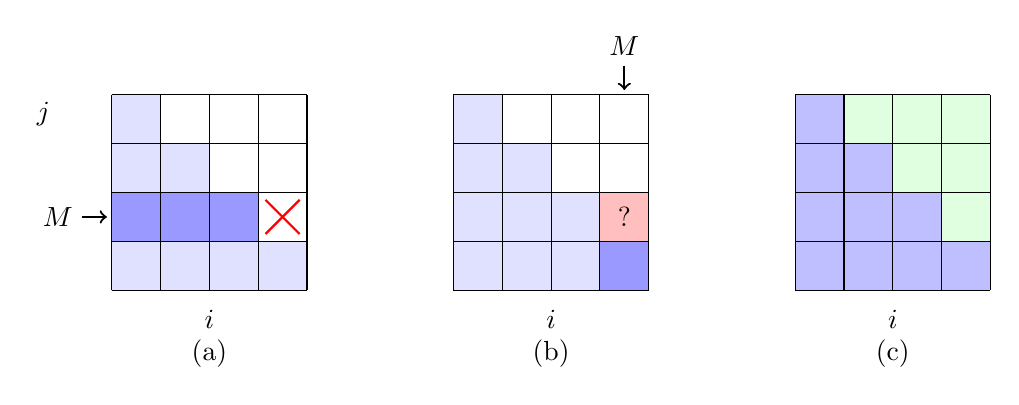
\begin{tikzpicture}[scale=0.62]
% ---------- panel (a): naive sweep along axis 1 pushes a value out of A
\begin{scope}
\foreach \i/\j in {0/0,1/0,2/0,3/0,0/1,1/1,2/1,0/2,1/2,0/3}{\fill[blue!12] (\i,\j) rectangle ++(1,1);}
\foreach \i in {0,1,2}{\fill[blue!40] (\i,1) rectangle ++(1,1);}
\draw[red,thick] (3.15,1.15) -- (3.85,1.85); \draw[red,thick] (3.15,1.85) -- (3.85,1.15);
\draw[step=1] (0,0) grid (4,4);
\draw[->,thick] (-0.6,1.5) -- (-0.1,1.5); \node[left] at (-0.6,1.5) {$M$};
\node at (2,-0.6) {$i$}; \node at (-1.4,3.6) {$j$};
\node at (2,-1.3) {(a)};
\end{scope}
% ---------- panel (b): sweep along axis 2 needs it
\begin{scope}[xshift=7cm]
\foreach \i/\j in {0/0,1/0,2/0,3/0,0/1,1/1,2/1,0/2,1/2,0/3}{\fill[blue!12] (\i,\j) rectangle ++(1,1);}
\fill[blue!40] (3,0) rectangle ++(1,1);
\fill[red!25] (3,1) rectangle ++(1,1); \node at (3.5,1.5) {?};
\draw[step=1] (0,0) grid (4,4);
\draw[->,thick] (3.5,4.6) -- (3.5,4.1); \node[above] at (3.5,4.6) {$M$};
\node at (2,-0.6) {$i$};
\node at (2,-1.3) {(b)};
\end{scope}
% ---------- panel (c): keep the pushed values
\begin{scope}[xshift=14cm]
\foreach \i in {0,...,3}\foreach \j in {0,...,3}{\fill[green!12] (\i,\j) rectangle ++(1,1);}
\foreach \i/\j in {0/0,1/0,2/0,3/0,0/1,1/1,2/1,0/2,1/2,0/3}{\fill[blue!25] (\i,\j) rectangle ++(1,1);}
\draw[step=1] (0,0) grid (4,4);
\node at (2,-0.6) {$i$};
\node at (2,-1.3) {(c)};
\end{scope}
\end{tikzpicture}
\caption{Two dimensions, $n=4$, $A=\{i+j\le3\}$ (blue). (a)~Sweep along axis $i$, row $j=1$: three inputs, four
outputs; the naive route drops the value at $(3,1)$ (red cross). (b)~Sweep along axis $j$, column $i=3$: its output at
$(3,0)\in A$ needs the input at $(3,1)$, which was dropped. (c)~Exact: after sweep~1 keep all $16$ values (green), sweep
the full columns, then crop to $A$ (blue). In 2D the product set $\pr{1}(A)\times\pr{2}(A)$ \emph{is} the box.}\label{fig:2d}
\end{figure}

\paragraph{Why the naive route breaks (Figure~\ref{fig:2d}).} Row $j=1$ has three entries inside $A$. Multiplying
them by $M$ gives four numbers; the fourth belongs to the cell $(3,1)$, outside $A$. The naive route has nowhere to
put it and drops it. The second sweep then multiplies column $i=3$ by $M$; its output at $(3,0)$, a point of $A$, is a
combination of all four entries of that column, including the dropped one. So the first sweep pushes values out of
$A$ and the second sweep needs them back. Keeping the full rows (panel~(c)) repairs this; in two dimensions the
repaired intermediate is the whole box.

\begin{figure}[ht]\centering
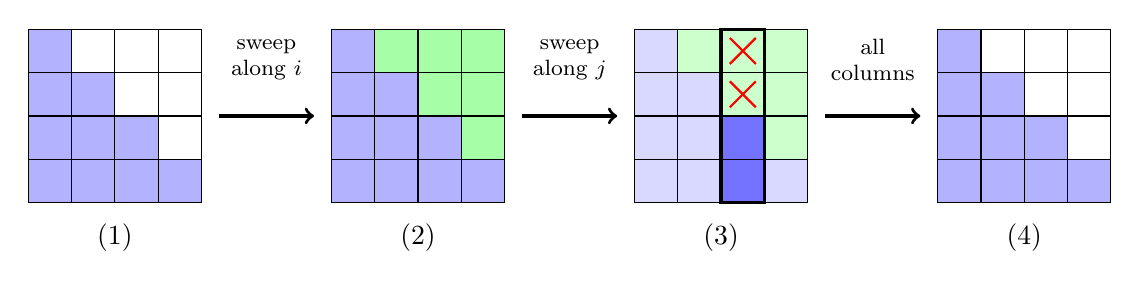
\begin{tikzpicture}[x=0.55cm,y=0.55cm]
\newcommand{\Acells}[1]{\foreach \i/\j in {0/0,1/0,2/0,3/0,0/1,1/1,2/1,0/2,1/2,0/3}{\fill[#1] (\i,\j) rectangle ++(1,1);}}
\newcommand{\Ocells}[1]{\foreach \i/\j in {1/3,2/2,2/3,3/1,3/2,3/3}{\fill[#1] (\i,\j) rectangle ++(1,1);}}
\newcommand{\cross}[2]{\draw[red,thick] (#1+0.2,#2+0.2) -- ++(0.6,0.6); \draw[red,thick] (#1+0.8,#2+0.2) -- ++(-0.6,0.6);}
\begin{scope}
\Acells{blue!30} \draw[step=1] (0,0) grid (4,4); \node at (2,-0.8) {(1)};
\end{scope}
\draw[->,very thick] (4.4,2) -- (6.6,2); \node[align=center,font=\footnotesize] at (5.5,3.3) {sweep\\ along $i$};
\begin{scope}[shift={(7,0)}]
\Acells{blue!30} \Ocells{green!35} \draw[step=1] (0,0) grid (4,4); \node at (2,-0.8) {(2)};
\end{scope}
\draw[->,very thick] (11.4,2) -- (13.6,2); \node[align=center,font=\footnotesize] at (12.5,3.3) {sweep\\ along $j$};
\begin{scope}[shift={(14,0)}]
\Acells{blue!15} \Ocells{green!20}
\fill[blue!55] (2,0) rectangle ++(1,2); \cross{2}{2} \cross{2}{3}
\draw[step=1] (0,0) grid (4,4); \draw[very thick] (2,0) rectangle (3,4); \node at (2,-0.8) {(3)};
\end{scope}
\draw[->,very thick] (18.4,2) -- (20.6,2); \node[align=center,font=\footnotesize] at (19.5,3.3) {all\\ columns};
\begin{scope}[shift={(21,0)}]
\Acells{blue!30} \draw[step=1] (0,0) grid (4,4); \node at (2,-0.8) {(4)};
\end{scope}
\end{tikzpicture}
\caption{The exact route in 2D, step by step ($n=4$, $A=\{i+j\le3\}$). (1)~Input $c$ on $A$ (blue), zeros outside. (2)~The sweep
along $i$ multiplies every row by the full $M$ and spreads it over all four columns; green = new nonzeros outside $A$; since
every value of $i$ occurs in $A$, no output is dropped and the array fills the box. (3)~The sweep along $j$, shown for column
$i=2$ (thick frame): the input is the full column of four values, but only the outputs with $j\le1$ (dark blue) are computed,
because $(2,j)\in A$ only for $j\le1$; the outputs at $(2,2)$, $(2,3)$ (red crosses) are not computed: coordinate $i$ is already
processed, no later sweep can change it, so they could never reach $A$. (4)~After all columns: exactly $A$. Dropping is
never a subtraction or a correction; it is not computing outputs that no later sweep can use.}\label{fig:steps}
\end{figure}

\paragraph{When and how entries are dropped.} Two rules, applied in every sweep along axis $k$:
\begin{itemize}
\item \emph{Input side, nothing to decide.} The input tube is the current set's tube; entries outside it are exactly
      zero (the forward fact below), so they are neither stored nor read. The zero padding in Figure~\ref{fig:kernel} is
      this rule.
\item \emph{Output side, this is where dropping happens.} After the multiplication the tube has $n$ outputs. Coordinates
      $1..k$ are now all processed and no later sweep changes them. An output whose coordinates $1..k$ do not form the
      beginning of some point of $A$ can never reach $A$, so it is not computed: the kernel is cut to $L_{\rm out}$ rows.
      In the first sweep this cuts nothing (every $i$ occurs in $A$); in the last sweep it cuts down to $A$'s own tubes,
      which is how the result lands on $A$.
\end{itemize}
Between the two rules, the values pushed outside $A$ by a sweep are neither removed nor moved back: they sit in the
enlarged set, are read by the next sweep as part of a full tube, and are then left behind because the next sweep's
outputs are computed only where they can still matter.

\paragraph{Why the box is more than needed for $m\ge3$.} Two facts about the array after $k$ sweeps:
\begin{itemize}
\item \emph{Forward:} a sweep along axis $k$ only mixes entries along axis $k$; it cannot create a nonzero entry in a
      slice (fixed coordinates $k{+}1,\dots,m$) that was empty. So after $k$ sweeps the nonzero entries sit only where
      the \emph{last} $m-k$ coordinates are the tail of some point of $A$.
\item \emph{Backward:} the remaining sweeps (axes $k{+}1,\dots,m$) only mix along those axes; the final value at a point
      $\alpha\in A$ can only come from entries whose \emph{first} $k$ coordinates equal $\alpha$'s. So entries whose first
      $k$ coordinates do not begin some point of $A$ can never reach $A$ and may be dropped.
\end{itemize}
Keep exactly the entries that are neither provably zero nor provably unused: first $k$ coordinates from the
projection of $A$ onto axes $1..k$, last $m-k$ coordinates from the projection onto axes $k{+}1..m$, with \emph{no joint
constraint between the two halves}. That is the product set $\pr{\le k}(A)\times\pr{>k}(A)$. Figure~\ref{fig:3d} shows it for
$m=3$: the box has $27$ cells, $A$ has $10$, each product set $18$.

\begin{figure}[ht]\centering
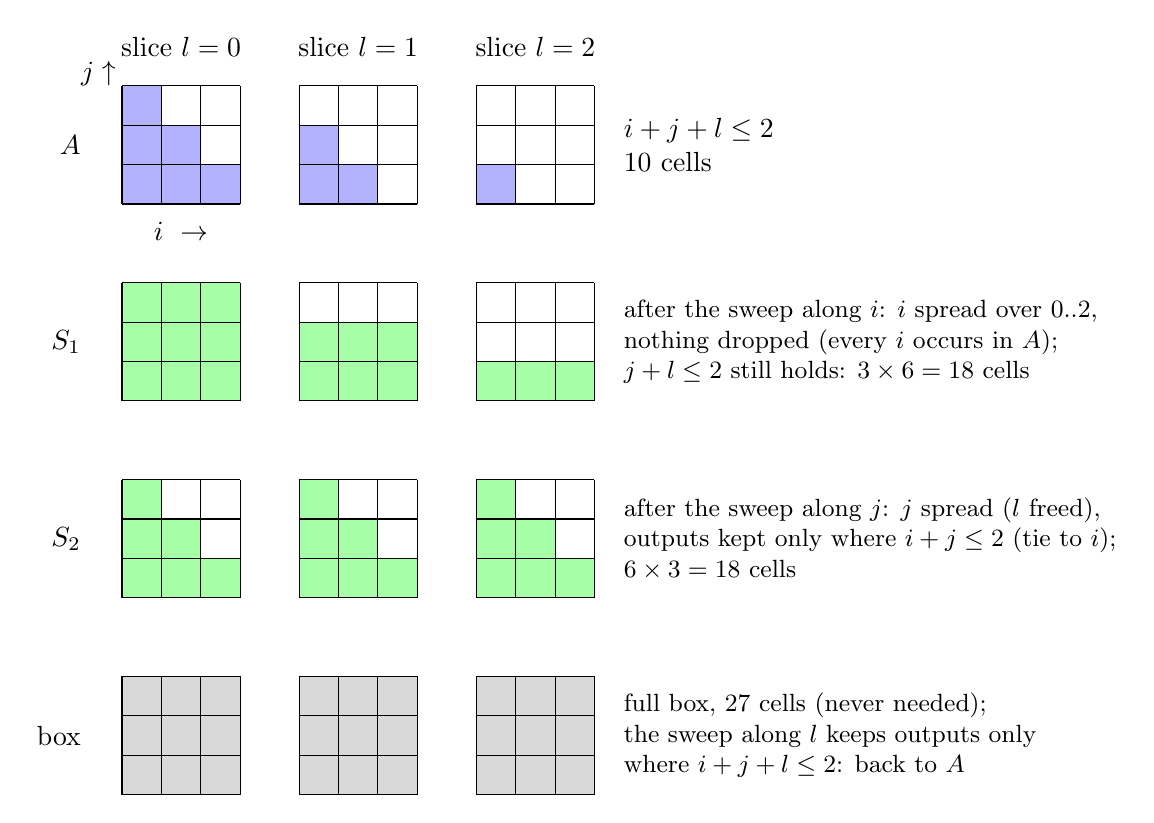
\begin{tikzpicture}[scale=0.5]
\newcommand{\gridthree}{\draw[step=1] (0,0) grid (3,3);}
% row labels
\node[left] at (-0.8,1.5) {$A$};
\node[left] at (-0.8,-3.5) {$S_1$};
\node[left] at (-0.8,-8.5) {$S_2$};
\node[left] at (-0.8,-13.5) {box};
\foreach \l in {0,1,2}{\node at (\l*4.5+1.5,4.0) {slice $l=\l$};}
% A: l=0: i+j<=2 ; l=1: i+j<=1 ; l=2: (0,0)
\begin{scope}
\foreach \i/\j in {0/0,1/0,2/0,0/1,1/1,0/2}{\fill[blue!30] (\i,\j) rectangle ++(1,1);} \gridthree
\end{scope}
\begin{scope}[xshift=4.5cm]
\foreach \i/\j in {0/0,1/0,0/1}{\fill[blue!30] (\i,\j) rectangle ++(1,1);} \gridthree
\end{scope}
\begin{scope}[xshift=9cm]
\foreach \i/\j in {0/0}{\fill[blue!30] (\i,\j) rectangle ++(1,1);} \gridthree
\end{scope}
\node[right,align=left] at (12.5,1.5) {$i+j+l\le2$\\ $10$ cells};
% S_1 = {j + l <= 2}: l=0: all 9 ; l=1: j<=1 ; l=2: j=0
\begin{scope}[yshift=-5cm]
\foreach \i in {0,1,2}\foreach \j in {0,1,2}{\fill[green!35] (\i,\j) rectangle ++(1,1);} \gridthree
\end{scope}
\begin{scope}[xshift=4.5cm,yshift=-5cm]
\foreach \i in {0,1,2}\foreach \j in {0,1}{\fill[green!35] (\i,\j) rectangle ++(1,1);} \gridthree
\end{scope}
\begin{scope}[xshift=9cm,yshift=-5cm]
\foreach \i in {0,1,2}{\fill[green!35] (\i,0) rectangle ++(1,1);} \gridthree
\end{scope}
\node[right,align=left,font=\small] at (12.5,-3.5) {after the sweep along $i$: $i$ spread over $0..2$,\\ nothing dropped (every $i$ occurs in $A$);\\ $j+l\le2$ still holds: $3\times6=18$ cells};
% S_2 = {i + j <= 2} x any l
\foreach \s in {0,1,2}{
\begin{scope}[xshift=\s*4.5cm,yshift=-10cm]
\foreach \i/\j in {0/0,1/0,2/0,0/1,1/1,0/2}{\fill[green!35] (\i,\j) rectangle ++(1,1);} \gridthree
\end{scope}}
\node[right,align=left,font=\small] at (12.5,-8.5) {after the sweep along $j$: $j$ spread ($l$ freed),\\ outputs kept only where $i+j\le2$ (tie to $i$);\\ $6\times3=18$ cells};
% box
\foreach \s in {0,1,2}{
\begin{scope}[xshift=\s*4.5cm,yshift=-15cm]
\foreach \i in {0,1,2}\foreach \j in {0,1,2}{\fill[gray!30] (\i,\j) rectangle ++(1,1);} \gridthree
\end{scope}}
\node[right,align=left,font=\small] at (12.5,-13.5) {full box, $27$ cells (never needed);\\ the sweep along $l$ keeps outputs only\\ where $i+j+l\le2$: back to $A$};
\node at (1.5,-0.7) {$i\ \rightarrow$}; \node at (-0.6,3.3) {$j\uparrow$};
\end{tikzpicture}
\caption{Three dimensions, $n=3$, $A=\{i+j+l\le2\}$, drawn as the three slices $l=0,1,2$ (axis $i$ horizontal, $j$ vertical).
Rows: the set $A$ where the input and the output live; the product set $S_1=\pr{1}(A)\times\pr{23}(A)$ where the array lives
after the sweep along $i$ (every slice shape of $A$ in $(j,l)$, but $i$ unconstrained); the product set
$S_2=\pr{12}(A)\times\pr{3}(A)$ after the sweep along $j$ (the triangle in $(i,j)$ in every slice, $l$ unconstrained); and the box.
The sweep along $l$ maps $S_2$ back to $A$.}\label{fig:3d}
\end{figure}

\paragraph{The three sweeps of Figure~\ref{fig:3d}, counted.}
\begin{enumerate}
\item Along $i$: a tube is ``fix $(j,l)$, vary $i$''; there are $6$ (the pairs with $j+l\le2$), with $3,2,2,1,1,1$ entries. Zero-pad
      each to length $3$, multiply by the full $3\times3$ matrix $M$, keep all $3$ outputs. The array now lives on $S_1$: $18$ cells.
      Cost $3\cdot(3+2+2+1+1+1)=30$ multiply--adds.
\item Along $j$: a tube is ``fix $(i,l)$, vary $j$''. Its input has the $j$ with $j+l\le2$ (length $3-l$, from $S_1$), its output
      needs the $j$ with $i+j\le2$ (length $3-i$, from $S_2$); the kernel is the top-left $(3-i)\times(3-l)$ block of $M$.
      Cost $\sum_{i,l}(3-i)(3-l)=36$. The array now lives on $S_2$: $18$ cells.
\item Along $l$: a tube is ``fix $(i,j)$, vary $l$'', $6$ tubes, input length $3$ (full, from $S_2$), output length $3-i-j$ ($A$'s own
      tube); kernel: top-left $(3-i-j)\times3$ block of $M$. Cost $30$. Result: the $10$ entries of $A$.
\end{enumerate}
Total $96$ multiply--adds, against $243$ for the box and $90$ for the two triangular LU sweeps. Here the price of not
needing any factorisation is seven percent.

\begin{figure}[ht]\centering
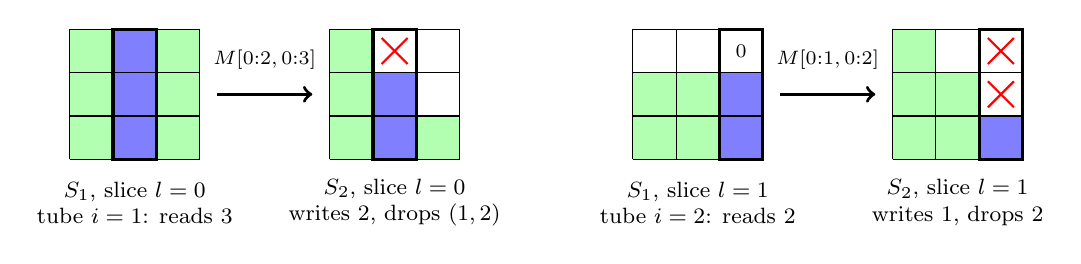
\begin{tikzpicture}[x=0.55cm,y=0.55cm]
\newcommand{\gridthree}{\draw[step=1] (0,0) grid (3,3);}
\newcommand{\cross}[2]{\draw[red,thick] (#1+0.2,#2+0.2) -- ++(0.6,0.6); \draw[red,thick] (#1+0.8,#2+0.2) -- ++(-0.6,0.6);}
\begin{scope}
\foreach \i in {0,1,2}\foreach \j in {0,1,2}{\fill[green!30] (\i,\j) rectangle ++(1,1);}
\fill[blue!50] (1,0) rectangle ++(1,3); \gridthree \draw[very thick] (1,0) rectangle (2,3);
\node[align=center,font=\footnotesize] at (1.5,-1.0) {$S_1$, slice $l=0$\\ tube $i=1$: reads 3};
\end{scope}
\draw[->,very thick] (3.4,1.5) -- (5.6,1.5); \node[font=\scriptsize] at (4.5,2.3) {$M[0{:}2,0{:}3]$};
\begin{scope}[shift={(6,0)}]
\foreach \i/\j in {0/0,1/0,2/0,0/1,1/1,0/2}{\fill[green!30] (\i,\j) rectangle ++(1,1);}
\fill[blue!50] (1,0) rectangle ++(1,2); \cross{1}{2} \gridthree \draw[very thick] (1,0) rectangle (2,3);
\node[align=center,font=\footnotesize] at (1.5,-1.0) {$S_2$, slice $l=0$\\ writes 2, drops $(1,2)$};
\end{scope}
\begin{scope}[shift={(13,0)}]
\foreach \i in {0,1,2}\foreach \j in {0,1}{\fill[green!30] (\i,\j) rectangle ++(1,1);}
\fill[blue!50] (2,0) rectangle ++(1,2); \gridthree \draw[very thick] (2,0) rectangle (3,3);
\node[font=\scriptsize] at (2.5,2.5) {$0$};
\node[align=center,font=\footnotesize] at (1.5,-1.0) {$S_1$, slice $l=1$\\ tube $i=2$: reads 2};
\end{scope}
\draw[->,very thick] (16.4,1.5) -- (18.6,1.5); \node[font=\scriptsize] at (17.5,2.3) {$M[0{:}1,0{:}2]$};
\begin{scope}[shift={(19,0)}]
\foreach \i/\j in {0/0,1/0,2/0,0/1,1/1,0/2}{\fill[green!30] (\i,\j) rectangle ++(1,1);}
\fill[blue!50] (2,0) rectangle ++(1,1); \cross{2}{1} \cross{2}{2} \gridthree \draw[very thick] (2,0) rectangle (3,3);
\node[align=center,font=\footnotesize] at (1.5,-1.0) {$S_2$, slice $l=1$\\ writes 1, drops 2};
\end{scope}
\end{tikzpicture}
\caption{Two tubes of the middle sweep (along $j$) of Figure~\ref{fig:3d}; axis $i$ horizontal, $j$ vertical, one slice $l$ per
grid, green = the set, thick frame = the tube. Left pair: in slice $l=0$ the tube $i=1$ reads three values (the whole column of
$S_1$, $L_{\rm in}=3-l=3$) and writes two ($L_{\rm out}=3-i=2$), because $(1,j)\in\pr{12}(A)$ only for $j\le1$; the third output
(red cross) is not computed. Right pair: in slice $l=1$ the tube $i=2$ reads two values ($S_1$ has $j+l\le2$; the cell $(2,2,1)$ is
exactly zero and is not read) and writes one. Input lengths come from the unprocessed coordinate $l$, output lengths from the
processed coordinate $i$; the kernel is the corresponding top-left block of $M$.}\label{fig:tube3d}
\end{figure}

\begin{figure}[ht]\centering
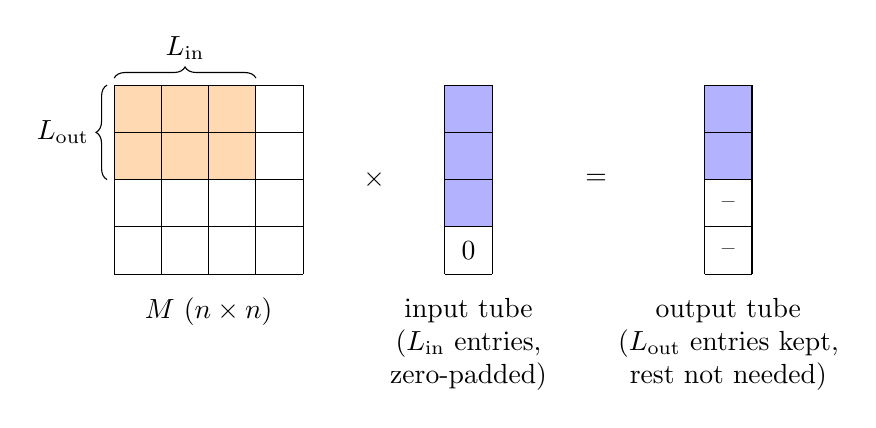
\begin{tikzpicture}[scale=0.6]
% matrix M with block
\fill[orange!30] (0,2) rectangle (3,4);
\draw[step=1] (0,0) grid (4,4);
\node[anchor=north] at (2,-0.3) {$M$ ($n\times n$)};
\draw[decorate,decoration={brace,amplitude=4pt}] (0,4.15) -- (3,4.15) node[midway,above=3pt] {$L_{\rm in}$};
\draw[decorate,decoration={brace,amplitude=4pt}] (-0.15,2) -- (-0.15,4) node[midway,left=3pt] {$L_{\rm out}$};
% input vector
\begin{scope}[xshift=7cm]
\fill[blue!30] (0,1) rectangle (1,4); \draw[step=1] (0,0) grid (1,4);
\node at (0.5,0.5) {$0$};
\node[align=center,anchor=north] at (0.5,-0.3) {input tube\\ ($L_{\rm in}$ entries,\\ zero-padded)};
\end{scope}
\node at (5.5,2) {$\times$};
% output vector
\begin{scope}[xshift=12.5cm]
\fill[blue!30] (0,2) rectangle (1,4); \draw[step=1] (0,0) grid (1,4);
\node[font=\small] at (0.5,1.5) {--}; \node[font=\small] at (0.5,0.5) {--};
\node[align=center,anchor=north] at (0.5,-0.3) {output tube\\ ($L_{\rm out}$ entries kept,\\ rest not needed)};
\end{scope}
\node at (10.2,2) {$=$};
\end{tikzpicture}
\caption{The tube kernel: only the top-left $L_{\rm out}\times L_{\rm in}$ block of $M$ acts. $L_{\rm in}$ is the tube length of the
current set (set by $A$'s shape in the not-yet-processed coordinates), $L_{\rm out}$ the tube length of the next set (set by $A$'s
shape in the already-processed coordinates). First sweep: $L_{\rm out}=n$ (zero-pad and multiply by all of $M$); last sweep:
$L_{\rm in}=n$ (multiply by all of $M$ and truncate); middle sweeps trim both ends. If $M$ has a fast algorithm, zero-pad to $n$,
transform, truncate.}\label{fig:kernel}
\end{figure}

\paragraph{The rule in one sentence.} Sweep $M$ itself, direction by direction; a tube's input length is set by $A$'s
shape in the not-yet-processed coordinates, its output length by $A$'s shape in the already-processed coordinates,
and the kernel is the corresponding top-left block of $M$ (Figure~\ref{fig:kernel}). Nothing is factorised, so nothing
can be unstable; each step is an ordinary matrix times vector. The naive route drops needed numbers, the box route
drops nothing and stores everything, the product-set route drops exactly the numbers that are provably zero or
provably unused. What the intermediate array does not need to remember is the \emph{joint} constraint of $A$ between
processed and unprocessed coordinates, only the two marginal shapes; that is why it is a product, and why it is much
smaller than the box as soon as $m\ge3$.

\section{Why LU works: the cropping lemma}
The FNT rests on two elementary facts, recorded here because the general principle of the next section
contains them as special cases.
\begin{lemma}[cropping lemma]\label{lem:crop}
Let $A$ be downward closed.
(i) If $U$ is upper triangular, $U^{\otimes m}$ maps $A$-supported vectors to $A$-supported vectors; hence
$\PA U^{\otimes m}\EA$ equals the $m$ sweeps of $U$ on the tubes of $A$, and nothing outside $A$ is created.
(ii) If $L$ is lower triangular, the $A$-part of $L^{\otimes m}x$ depends only on the $A$-part of $x$; hence
$\PA L^{\otimes m}\EA$ equals the $m$ sweeps of $L$ on the tubes of $A$, and nothing outside $A$ is needed.
\end{lemma}
\begin{proof}
(i) $(Ux)_i=\sum_{j\ge i}U_{ij}x_j$: output index $\le$ input index in every coordinate, so if $\beta$ receives a
contribution from $\alpha\in A$ then $\beta\le\alpha$ and $\beta\in A$. (ii) $(Lx)_i=\sum_{j\le i}L_{ij}x_j$: the output at
$\alpha\in A$ uses inputs at $\beta\le\alpha$, all in $A$.
\end{proof}
Consequently $\KA(LU)=\PA L^{\otimes m}\EA\cdot\PA U^{\otimes m}\EA$: apply the $U$-sweeps first (their output stays in $A$),
then the $L$-sweeps (they need nothing outside $A$). The order is forced: an $L$-sweep followed by a $U$-sweep is
the failure of Section~\ref{sec:naive}. The theory thread proved the converse: a scheme of square sweeps on $A$
built from a fixed factorisation of $M$, valid for every downward closed $A$, exists if and only if $M$ has an
unpivoted LU (\texttt{explore/theory/REPORT.md}, T2). So for a general $M$ we must leave $A$.

\section{The needed-set principle}\label{sec:needed}
Nothing forces the intermediate results to live on $A$. We apply the exact mode products
$v_0=\EA c$, $v_k=M_{(k)}v_{k-1}$ ($k=1,\dots,m$), $y=\PA v_m$, and ask on which set each $v_k$ has to be
\emph{known}. Two sets answer this. For $S\subset\{1,\dots,m\}$ let $\pr{S}$ denote the projection of a multi-index
onto the coordinates in $S$, and $\pr{S}(A)$ the projection of the set.

\begin{definition}[push-forward and pull-back]
\begin{align*}
 \mathrm{Push}_k&:=\{\beta\in B:\ \pr{>k}(\beta)\in\pr{>k}(A)\},\\
 \mathrm{Need}_k&:=\{\beta\in B:\ \pr{\le k}(\beta)\in\pr{\le k}(A)\},\\
 S_k&:=\mathrm{Push}_k\cap\mathrm{Need}_k=\pr{\le k}(A)\times\pr{>k}(A).
\end{align*}
\end{definition}
$\mathrm{Push}_k$ is where $v_k$ can be nonzero: the sweeps done so far ($1,\dots,k$) only moved mass along the first $k$
coordinates, so the last $m-k$ coordinates of any nonzero entry still match a point of $A$. $\mathrm{Need}_k$ is
where $v_k$ is needed: the sweeps still to come ($k+1,\dots,m$) only move mass along the last $m-k$ coordinates,
so an output point $\alpha\in A$ is reached only from entries whose first $k$ coordinates equal $\pr{\le k}(\alpha)$.
Note $S_0=A$, $S_m=A$, and each $S_k$ is a Cartesian product of two downward closed sets, hence downward closed.

\begin{theorem}[product-set sweeps]\label{thm:main}
Define $w_0=\EA c$ and, for $k=1,\dots,m$,
\[
 w_k(\beta)=\begin{cases}\displaystyle\sum_{\gamma:\ \beta[k\to\gamma]\in S_{k-1}} M_{\beta_k,\gamma}\,w_{k-1}(\beta[k\to\gamma]) & \beta\in S_k,\\[1ex] 0 & \beta\notin S_k,\end{cases}
\]
where $\beta[k\to\gamma]$ is $\beta$ with its $k$-th coordinate replaced by $\gamma$. Then $w_k=v_k$ on $S_k$ for every $k$, and
$y=\KA(M)c=\PA w_m$. Every entry of $w_k$ outside $S_k$ that is thereby discarded is either zero or never used.
\end{theorem}
\begin{proof}
Three observations. (a) $\supp v_k\subset\mathrm{Push}_k$: by induction, $v_k(\beta)\ne0$ needs some $\gamma$ with
$\beta[k\to\gamma]\in\mathrm{Push}_{k-1}$, i.e. $(\gamma,\pr{>k}\beta)\in\pr{\ge k}(A)$, hence $\pr{>k}\beta\in\pr{>k}(A)$.
(b) If $\beta\in\mathrm{Need}_k$ then $\beta[k\to\gamma]\in\mathrm{Need}_{k-1}$ for every $\gamma$: the first $k-1$ coordinates
of $\beta[k\to\gamma]$ are those of $\beta$, and $\pr{<k}\beta$ is the projection of the point $\pr{\le k}\beta\in\pr{\le k}(A)$.
(c) $\PA v_m$ uses $v_m$ only on $A=\mathrm{Need}_m$.
Now induct on $k$: assume $w_{k-1}=v_{k-1}$ on $S_{k-1}$ (true for $k=1$). For $\beta\in S_k$ the exact value is
$v_k(\beta)=\sum_{\gamma}M_{\beta_k\gamma}v_{k-1}(\beta[k\to\gamma])$ over all $\gamma$. Terms with $\beta[k\to\gamma]\notin\mathrm{Push}_{k-1}$
vanish by (a). Since $\beta\in\mathrm{Need}_k$, every $\beta[k\to\gamma]$ lies in $\mathrm{Need}_{k-1}$ by (b). So every nonzero term
has $\beta[k\to\gamma]\in S_{k-1}$, where $w_{k-1}=v_{k-1}$; the two sums agree. Finally $y=\PA v_m=\PA w_m$ by (c) and $S_m=A$.
\end{proof}

\begin{remark}[tightness and the naive route]
For a generic (dense) $M$ the sets $S_k$ are minimal: removing any single point of any $S_k$ changes the result
(checked on $1034$ of $1034$ removals, \texttt{explore/theory/REPORT.md}, T3, and \texttt{explore/skeptic/results.md},
claim~2). The naive route of Section~\ref{sec:naive} is Theorem~\ref{thm:main} with $S_k$ replaced by $A$; it is exact iff
no nonzero term is dropped, which for generic entries means $M$ upper triangular (this is the ``chain criterion'' of
Valentin's 2019 thesis, arXiv:1910.05379, Prop.~4.24, as the special case of one sweep per direction). The
cropping lemma is the same principle: for upper $U$, $\supp v_k\subset A$ so $S_k$ may be shrunk to $A$; for lower $L$,
$\mathrm{Need}_k$ may be shrunk to $A$.
\end{remark}

\section{The algorithm}\label{sec:algo}
Theorem~\ref{thm:main} is a sweep algorithm with \emph{rectangular} tube kernels. Fix the direction $k$ and all
coordinates except the $k$-th: $a=\pr{<k}(\beta)$, $b=\pr{>k}(\beta)$. The input array $w_{k-1}$ lives on
$S_{k-1}=\pr{<k}(A)\times\pr{\ge k}(A)$, so the input tube $(a,\cdot,b)$ is nonempty iff $a\in\pr{<k}(A)$ and $b\in\pr{>k}(A)$,
and it is the prefix of length
\[
 L_{\rm in}(b)=\#\{\gamma:\ (\gamma,b)\in\pr{\ge k}(A)\}.
\]
The output array $w_k$ lives on $S_k=\pr{\le k}(A)\times\pr{>k}(A)$, so the output tube is the prefix of length
\[
 L_{\rm out}(a)=\#\{\gamma:\ (a,\gamma)\in\pr{\le k}(A)\}.
\]
Both are prefixes because the projections of a downward closed set are downward closed. The tube kernel is
\begin{equation}\label{eq:kernel}
 w_k(a,0{:}L_{\rm out},b)\;=\;M[\,0{:}L_{\rm out}(a),\ 0{:}L_{\rm in}(b)\,]\;\,w_{k-1}(a,0{:}L_{\rm in},b).
\end{equation}
\begin{center}
\begin{tabular}{@{}p{0.95\textwidth}@{}}
\toprule
\textbf{Algorithm} (product-set sweeps for $y=\PA M^{\otimes m}\EA c$)\\
\midrule
1. $w\leftarrow c$ on $A$ (zero elsewhere).\\
2. For $k=1,\dots,m$: for every pair $a\in\pr{<k}(A)$, $b\in\pr{>k}(A)$ apply \eqref{eq:kernel} to the tube $(a,\cdot,b)$;
   the result lives on $S_k=\pr{\le k}(A)\times\pr{>k}(A)$.\\
3. $y\leftarrow w$ restricted to $A$ ($S_m=A$, nothing to crop).\\
\midrule
Fast variant: if $M$ has a fast algorithm (DCT-type, Toeplitz-type), replace \eqref{eq:kernel} by ``zero-pad the tube
to length $n$, apply $M$ fast, keep the first $L_{\rm out}$ entries''.\ \ Per-direction matrices: use $M^{(k)}$ in step $k$.\\
\bottomrule
\end{tabular}
\end{center}
Three special cases are worth seeing.
\begin{itemize}
\item \textbf{First sweep} ($k=1$): $L_{\rm in}$ is the tube length of $A$ and $L_{\rm out}=|\pr{1}(A)|=n$ for any set
      that contains $(n-1,0,\dots,0)$. So the first sweep is ``zero-pad every tube of $A$ to full length and apply the
      whole $M$''.
\item \textbf{Last sweep} ($k=m$): $L_{\rm in}=n$ and $L_{\rm out}$ is the tube length of $A$: ``apply the whole $M$ and truncate''.
\item \textbf{Middle sweeps} have both a shortened input ($L_{\rm in}$ set by the later coordinates $b$) and a shortened
      output ($L_{\rm out}$ set by the earlier coordinates $a$).
\end{itemize}
\begin{example}[2D triangle]
$m=2$, $n=4$, $A=\{(i,j): i+j\le3\}$. Sweep~1 (direction $1$, columns $j$): the column $j$ is a tube of $A$ of length
$L_{\rm in}=4-j$; the output set $S_1=\pr{1}(A)\times\pr{2}(A)=\{0..3\}^2$ is the whole box, $L_{\rm out}=4$; kernel
$M[0{:}4,0{:}4-j]$. Sweep~2 (direction $2$, rows $i$): $L_{\rm in}=4$, output $A$ with $L_{\rm out}=4-i$; kernel $M[0{:}4-i,0{:}4]$.
In two dimensions $S_1$ is always the bounding box (both projections are full), so the product-set route
\emph{is} the box route there; the saving over the box begins at $m=3$, where $S_1=\{0..n-1\}\times\pr{23}(A)$ and
$S_2=\pr{12}(A)\times\{0..n-1\}$ are cylinders over the 2D slices, each a few times $|A|$ while the box is
$n^3\gg|A|$. Applying Theorem~\ref{thm:main} to the counterexample of Section~\ref{sec:naive} keeps $v(1,1)=c\,c_{01}$
in $S_1=\{0,1\}^2$, and the second sweep produces the missing term $b\cdot c\,c_{01}$.
\end{example}

\section{Cost and memory}\label{sec:cost}
Summing \eqref{eq:kernel} over the tubes of sweep $k$ gives $\sum_{a}\sum_{b}L_{\rm out}(a)L_{\rm in}(b)=|\pr{\le k}(A)|\cdot|\pr{\ge k}(A)|$
multiply--adds, hence
\begin{equation}\label{eq:cost}
 \mathrm{flops}=\sum_{k=1}^{m}|\pr{\le k}(A)|\,|\pr{\ge k}(A)|,\qquad
 \mathrm{memory}=\max_{k}|S_k|=\max_k|\pr{\le k}(A)|\,|\pr{>k}(A)|,
\end{equation}
to be compared with the FNT ideal of $2m$ triangular sweeps on $A$ (about $2m\sum_{\rm tubes}L^2/2$) and the box
($m\,n^{m+1}$). For the symmetric families the projections are the lower-dimensional sets of the same family:
for the $\ell^1$ ball (total degree $\le n-1$) $|\pr{\le k}A|=|A^{(k)}|\approx n^k/k!$, so $|S_k|/|A|\approx\binom{m}{k}$ and the
total flop count is about $2^m n|A|$; for $\ell^2$ balls $|S_k|/|A|\approx V_kV_{m-k}/V_m$ with $V_j$ the volume of the
$j$-dimensional unit ball ($\approx2$ at $m=4$, $3.4$ at $m=6$, $11$ at $m=10$, $27$ at $m=13$), much smaller than
$\binom{m}{k}$. Measured ratios (cost model validated against enumeration on $32$ counts,
\texttt{explore/costmodel/results.md}; the shift thread's table \texttt{explore/shift/tables/x4\_cost.md}):

\begin{center}\small
\begin{tabular}{@{}p{2.2cm}p{2.0cm}p{3.2cm}p{1.5cm}p{4.9cm}@{}}
\toprule
set & $m$ ($n$) & flops / FNT ideal & memory / $|A|$ & comparison \\
\midrule
$\ell^2$ ball & $2$ / $3$ / $4$ ($8..64$) & $1.1$--$1.2$ / $1.3$--$1.4$ / $1.5$--$1.7$ & $\le2$ & $1.35$--$18\times$ cheaper than tracked $2^m$ splitting\\
$\ell^2$ ball & $13$ ($8$); $13$ ($16$) & $7.05$; $10.2$ & --; $19.6$ & shift route $18$--$27$\\
$\ell^2$ ball & $3$ ($1024$) & $1.4$ & $1.5$ & box $2.6$\\
$\ell^1$ ball & $2$ / $3$ / $4$ ($8..64$) & $1.3$--$1.5$ / $1.9$--$2.3$ / $2.8$--$3.7$ & $\binom{m}{\lfloor m/2\rfloor}$ & identical flops to tracked splitting on $\ell^1$ (observed for all cases, proved for $m=2$)\\
$\ell^1$ ball & $13$ ($8$); $13$ ($16$) & $25.6$; $82.7$ & $76$; $247$ & memory-bound: here the shift route ($18.5$, $5|A|$ memory) wins\\
hyperbolic cross & $\ge3$ & -- & up to $546$ & tracked splitting $1.3$--$11\times$ cheaper\\
random downward closed & $2..4$ & $0.96$--$1.63$ & -- & tracked splitting $1.5$--$6.7$\\
\bottomrule
\end{tabular}
\end{center}
\normalsize
With a fast 1D transform (kernel cost $\sim n\log n$ per tube instead of $L_{\rm out}L_{\rm in}$) the product-set route
beats even the \emph{dense} FNT ideal on $\ell^2$ balls from $n\approx16$--$32$ on, and on $\ell^1$ balls at $m=2$ for
$n\ge16$, $m=3$ for $n\ge64$, $m=4$ for $n\ge256$; never on hyperbolic crosses. The prototype
(\texttt{explore/prototype/REPORT.md}) measured $1.4$--$2.4\times$ FNT on $\ell^2$ balls with small $n$ and $m=4..6$.
An lpFun-friendly simplification is to use square sweeps on the single superset $D=\bigcup_kS_k$ (zero-pad $A\to D$,
sweep, crop): exact, $|D|/|A|=1.3$--$3.2$ on $\ell^2$ balls, $1.2$--$3\times$ the rectangular cost.

\section{Complexity: product sets versus unpivoted LU}\label{sec:cmp}
This section puts the two routes in the same currency and answers ``what does exactness for an arbitrary $M$
cost compared with the FNT when $M=LU$ happens to exist?''. We count multiply--adds; a dense $L_{\rm out}\times L_{\rm in}$
block costs $L_{\rm out}L_{\rm in}$, a triangular $L\times L$ block $L(L+1)/2$. Let $T_d$ be the set of tubes of $A$ in
direction $d$ and $L(t)$ the length of tube $t$; note $\sum_{t\in T_d}L(t)=|A|$ for every $d$.

\paragraph{Unpivoted LU (FNT).} Two triangular sweeps per direction on the tubes of $A$:
\begin{equation}\label{eq:clu}
 C_{LU}=\sum_{d=1}^{m}\sum_{t\in T_d}L(t)\big(L(t)+1\big)\ \approx\ \sum_{d=1}^m W_d,\qquad W_d:=\sum_{t\in T_d}L(t)^2,
\end{equation}
plus the one-off factorisation $\tfrac23n^3$. Memory: $|A|$ (in place). $W_d$ is the cost of one dense sweep on $A$'s own
tubes; since $L\le n$, $W_d\le n|A|$ with equality only when every tube is full.

\paragraph{Product sets.} One dense rectangular sweep per direction, \eqref{eq:cost}:
\[
 C_{PS}=\sum_{k=1}^{m}|\pr{\le k}(A)|\,|\pr{\ge k}(A)|,\qquad \text{memory }\max_k|\pr{\le k}(A)|\,|\pr{>k}(A)| .
\]
No factorisation. Per tube the first and last sweeps pay $n\cdot L$ instead of $L^2$: the price of exactness for a
general $M$ is that every tube is treated as if it were full length, because the sweep cannot know that the true
support would have stayed in $A$. The middle sweeps pay $L_{\rm out}L_{\rm in}$ with both factors shortened.

\paragraph{Closed forms.} On the full box both routes cost $m\,n^{m+1}$ and the ratio is $1$. On the $\ell^1$ ball of degree
$n-1$ (with $|A^{(j)}|\approx n^j/j!$ for $n\gg m$),
\begin{align*}
 C_{PS}&\approx n^{m+1}\sum_{k=1}^m\frac{1}{k!\,(m-k+1)!}=n^{m+1}\frac{2^{m+1}-2}{(m+1)!},\qquad
 C_{LU}\approx m\cdot\frac{2\,n^{m+1}}{(m+1)!},\\
 \frac{C_{PS}}{C_{LU}}&\ \longrightarrow\ \frac{2^m-1}{m}.
\end{align*}
On the $\ell^2$ ball, with $V_j=\pi^{j/2}/\Gamma(j/2+1)$ the volume of the $j$-dimensional unit ball,
$|\pr{\le k}A|\approx V_k(n/2)^k$ and $W_d\approx\int_{B_{m-1}}(n^2-r^2)=\frac{2}{m+1}V_{m-1}(n/2)^{m-1}n^2$, so
\[
 \frac{C_{PS}}{C_{LU}}\ \longrightarrow\ \frac{(m+1)\sum_{k=1}^{m}V_kV_{m-k+1}}{8\,m\,V_{m-1}} .
\]
The memory ratio tends to $\max_k\binom{m}{k}=\binom{m}{\lfloor m/2\rfloor}$ on $\ell^1$ balls and to $\max_kV_kV_{m-k}/V_m$ on $\ell^2$ balls.
The limits are approached from below (finite $n$ has fewer full-length tubes than the continuum count); they
require $n\gg m$, which is why the measured $\ell^1$ ratio at $m=13$ is $26$ ($n=8$) and $83$ ($n=16$) rather than $630$.

\begin{center}\small
\begin{tabular}{@{}lcccccc@{}}
\toprule
 & & \multicolumn{3}{c}{$C_{PS}/C_{LU}$, exact enumeration} & limit & memory$/|A|$ \\
set & $m$ & $n=8$ & $n=16$ & $n=32$ & $n\to\infty$ & ($n=32$; limit) \\
\midrule
$\ell^1$ ball & 2 & 1.20 & 1.33 & 1.41 & 1.50 & 1.94; 2 \\
$\ell^1$ ball & 3 & 1.62 & 1.92 & 2.11 & 2.33 & 2.82; 3 \\
$\ell^1$ ball & 4 & 2.20 & 2.79 & 3.21 & 3.75 & 5.32; 6 \\
$\ell^2$ ball & 2 & 1.08 & 1.11 & 1.15 & 1.18 & 1.31; 1.27 \\
$\ell^2$ ball & 3 & 1.19 & 1.30 & 1.35 & 1.41 & 1.50; 1.50 \\
$\ell^2$ ball & 4 & 1.36 & 1.54 & 1.62 & 1.72 & 1.93; 2.00 \\
box & 2--4 & 0.89 & 0.94 & 0.97 & 1 & 1; 1 \\
\midrule
\multicolumn{7}{@{}l@{}}{limits for $m=5,\dots,10$ and $m=13$:}\\
\multicolumn{7}{@{}l@{}}{\quad $\ell^1$ ratio $6.2,\,10.5,\,18,\,32,\,57,\,102$; $630$.\quad $\ell^1$ memory $10,20,35,70,126,252$; $1716$.}\\
\multicolumn{7}{@{}l@{}}{\quad $\ell^2$ ratio $2.1,\,2.6,\,3.3,\,4.2,\,5.4,\,6.9$; $15$.\quad $\ell^2$ memory $2.5,3.4,4.4,6.0,7.9,10.9$; $27$.}\\
\bottomrule
\end{tabular}
\end{center}
(Enumeration by \texttt{crop.py} on the actual sets; the box ratio is below $1$ only because \eqref{eq:clu} counts $L(L+1)$
for the two triangular sweeps against $L^2$ for one dense sweep.)

\paragraph{Reading the table.} In the FFT-paper regime ($m\le4$) exactness for an arbitrary $M$ costs $10$--$60\%$ more
than the FNT on $\ell^2$ balls and $1.2$--$3.2\times$ on $\ell^1$ balls, with at most twice ($\ell^2$) or six times ($\ell^1$)
the memory. In the thesis regime (large $m$, small $n$) the $\ell^2$ ratio stays moderate ($7$--$10$ at $m=13$) while the
$\ell^1$ ratio and above all the $\ell^1$ memory grow like $2^m/m$ and $\binom{m}{m/2}$: that is exactly where the
complex-shift route (about $18\times$ FNT, $5|A|$ memory) takes over. Hyperbolic crosses are worse still for product sets
(memory up to $546|A|$) and belong to the tracked splitting.

\paragraph{When $M$ is fast.} The LU factors of a fast matrix are dense triangular matrices, so the FNT cost
\eqref{eq:clu} is $\Theta(\sum_dW_d)$ whatever $M$ is. The product-set route inherits a fast $M$ because its kernel is a
leading block of $M$ (zero-pad, transform, truncate): the cost becomes $\sum_k|\pr{<k}A|\,|\pr{>k}A|\cdot c\,n\log_2n$, i.e.
$c\,n\log_2 n$ per tube instead of $L_{\rm out}L_{\rm in}\sim n^2$. On balls this beats the dense FNT from $n\approx16$--$32$ on
(costmodel thread, with $c\approx1.25$), so for DCT-type $M$ the generic route is not only exact but cheaper than the LU sweeps.

\paragraph{What the extra cost buys.} Compared with LU the product-set route (i) needs no $O(n^3)$ factorisation and no
pivot decision, (ii) is exact for every $M$, including rank-deficient and permutation-like matrices where the LU does not
exist, (iii) has the rounding error of a plain product (Section~\ref{sec:stab}) instead of $\KA(|L||U|)$, and (iv) is the
$w=n-1$ member of the bounded-delay family, so whenever a small delay suffices the same code with smaller sets
recovers the LU cost to within $1$--$25\%$ (delaypivot and hybrid threads).

\section{Stability}\label{sec:stab}
Every sweep is an ordinary matrix--vector product with a leading block of $M$; there are no pivots, no
multipliers and no cancellation between terms. The stability thread's shadow lemma
(\texttt{explore/stability/stability.pdf}, Lemma~2) applies to any chain of $K$ tube sweeps with factors $F_k$: if
$s$ denotes the result of the same chain run with $|F_k|$ on $|c|$, then in the absence of underflow and overflow
\[
 |\hat y-y|\ \le\ \big((1+\gamma_n)^K-1\big)\,s\quad\text{componentwise},\qquad \gamma_n\approx n\,\varepsilon .
\]
For the product-set sweeps the sets are exact for $|M|$ as well, so $s=\KA(|M|)\,|c|$ and, with $K=m$,
\[
 |\hat y-y|\le\big((1+\gamma_n)^m-1\big)\,\KA(|M|)|c|,\qquad \|\hat y-y\|_\infty\le m\gamma_n(1+\gamma_n)^{m-1}\|M\|_\infty^m\|c\|_\infty .
\]
This is the same bound as for the full box route and for the dense product $M^{\otimes m}$ itself, and it contains
no growth factor. By contrast the LU sweeps obey $|\hat y-y|\le2m\gamma_n\,\KA(|L||U|)|c|$, in which $|L||U|$ can exceed
$|M|$ arbitrarily when pivoting would have been needed. The shadow $s$ is also a rigorous a-posteriori error bound
at the price of one extra apply on non-negative data; the stability thread validated it on about $2750$ runs with
no violation. (The skeptic checked the product-set route itself for exactness, $39/39$ cases at $4.7\cdot10^{-17}$, but
no thread measured its rounding error against extended precision; the bound above is a one-line corollary of the
lemma and the theorem.)

\section{Relation to the other routes}\label{sec:rel}
\begin{itemize}
\item \textbf{Unpivoted LU} is the case where the sets can be shrunk back to $A$: $U$-sweeps have $\supp v_k\subset A$, $L$-sweeps
      need only $A$. Cost $2m$ triangular sweeps. Use it when GENP is backward stable (the positive definite convolution
      kernels of the thesis, for instance).
\item \textbf{Bounded-delay pivoting} ($M=L'U$ with $L'=PL$ lower plus $w$ superdiagonals) sits in between: $U$-sweeps on $A$,
      then $L'$-sweeps on sets thickened by $w$ in the unprocessed directions. For $w=n-1$ these sets are the product
      sets, so the product-set route is bounded-delay pivoting with unlimited delay and no factorisation.
\item \textbf{$2^m$ splitting} $M=T+B$ and the \textbf{complex-shift extrapolation} keep all intermediates on $A$ but use several
      chains or several matrices. Splitting wins on hyperbolic crosses; the shift wins only in the memory-bound
      $\ell^1$ cases $m\ge10$.
\item \textbf{$QR$.} With $M=QR$ one may sweep $R$ on $A$ (upper triangular) and then $Q$ on the product sets with
      $Q[0{:}L_{\rm out},0{:}L_{\rm in}]$. The $Q$ part costs exactly what sweeping $M$ costs, so $QR$ is a detour; orthogonality
      buys no stability here because the product-set route already has none of LU's growth.
\item \textbf{The solve} is not covered. $\det\KA(M)=\prod_k\det(M_k)^{e_k}$ with $e_k>0$ at the levels where the tube-length
      profile of $A$ steps down (\texttt{explore/theory/REPORT.md}, T6), so $\KA(M)$ is singular or ill-conditioned exactly
      when the unpivoted LU has a zero or tiny pivot at such a level; no forward route changes that.
\end{itemize}

\section{Verification record}
Exactness of Theorem~\ref{thm:main} was checked against the dense $|A|\times|A|$ operator and the full box route by three
independent codes: theory thread \texttt{verify.py} (the sets $S_k$ reproduce the tight sets; tightness $1034/1034$), prototype
(route \texttt{dense}, $43$ cases, error $\le2.5\cdot10^{-16}$; the automatic selector uses it as the fallback for the
natural-order DCT), skeptic (own mode-product reference, $39/39$ cases incl.\ $\ell^1$, $\ell^2$, hyperbolic cross, a
non-symmetric random set, a set touching the box boundary, a single long tube, different $n_d$ per direction,
$m=2..4$; error $\le4.7\cdot10^{-17}$). The flop formula \eqref{eq:cost} matches direct enumeration ($32$ counts, costmodel;
the skeptic corrected the symmetric-family form $\sum_j|A^{(j)}||A^{(m-j+1)}|$ to the general form above).

\section{Summary}
To apply an arbitrary $M$ across the modes of a downward closed $A$: sweep $M$ itself, direction by direction, with the
$k$-th intermediate kept on $\pr{\le k}(A)\times\pr{>k}(A)$ and the tube kernel $M[0{:}L_{\rm out},0{:}L_{\rm in}]$. It is exact for every
$M$ (Theorem~\ref{thm:main}), needs no factorisation and no pivoting, has the rounding error of a plain matrix product, costs
$\sum_k|\pr{\le k}A||\pr{\ge k}A|$ multiply--adds ($1.1$--$1.7\times$ the FNT on $\ell^2$ balls for $m\le4$, in two dimensions it is the
box route), and its only weakness is memory on $\ell^1$ balls at large $m$, where the middle sets reach $\binom{m}{m/2}|A|$.
\end{document}
